\chapter{Implementacija i korisničko sučelje}


\section{Korištene tehnologije i alati}

\text
Za potrebe komunikacije među članovima tima korištena je aplikacija \underline{WhatsApp}\footnote{https://www.whatsapp.com/}.
Za izradu UML dijagrama korišten je alat \underline{Astah Professional}\footnote{https://astah.net/products/astah-professional/},
a kao sustav za upravljanje izvornim kodom \underline{Git}\footnote{https://git-scm.com}.
Udaljeni repozitorij projekta dostupan je na web platformi \underline{GitLab}\footnote{https://about.gitlab.com}.

\text
Za razvojno okruženje odlučili smo se za \underline{Microsoft Visual Studio Code}\footnote{https://code.visualstudio.com}.
Visual Studio Code, ili kraće VSC, integrirano je razvojno okruženje (IDE) tvrtke Microsoft.
Značajke VSC-a uključuju podršku za otklanjanje pogrešaka, isticanje sintakse, inteligentno dovršavanje koda, isječke, refaktoriranje
koda i ugrađeni Git.

\text
Aplikacija je napisana koristeći radni okvir \underline{Spring Boot}\footnote{https://spring.io} i jezik
\underline{Java}\footnote{https://www.java.com/en/} za izradu \textit{backenda} te
\underline{React}\footnote{https://reactjs.org} i jezik \underline{TypeScript}\footnote{https://www.typescriptlang.org}
za izradu \textit{frontenda}.
React je biblioteka u JavaScriptu za izradu korisničkih sučelja. Održavaju ga Meta i zajednica pojedinačnih programera i tvrtki.
React se najčešće koristi kao osnova u razvoju web i mobilnih aplikacija.
React se bavi samo upravljanjem stanjem i prikazivanjem tog stanja te prilikom izrade složenijih aplikacija zahtjeva korištenje
dodatnih biblioteka za interakciju s API-jem.
Radni okvir Spring boot je sredstvo kojim se olakšava i ubrzava izrada web aplikacija.
Ima mogućnost autokonfiguracije, odlučan pristup konfiguraciji i mogućnost izrade samostalnih aplikacija.
Ove značajke rade zajedno kako bi vam pružile alat koji vam omogućuje postavljanje aplikacije koja se temelji na Springu uz minimalnu konfiguraciju i postavljanje.

\text
Baza podataka se nalazi na poslužitelju u oblaku na \underline{AWS}\footnote{https://aws.amazon.com/}


\eject


\section{Ispitivanje programskog rješenja}


\subsection{Ispitivanje komponenti}
Obavljeno je ispitavanje funkcionalnosti metoda iz klase: \textit{RecipeController.java}.
Poseban naglasak na metodi dodavanja novog recepta koja prima podatke
iz HTTP zahtjeva provjerava ih i priprema za spremanje u bazu.
Ta metoda se zove \linebreak\textit{+getNewRecipeData(RecipeRequest, User):RecipeData}
i nalazi se u razredu \textit{RecipeController.java}. Prvi ispitni slučaj je namijenjen provjeri sigurnosti
tako da se ne dopusti funkcionalnost dodavanja recepta neprijavljenim korisnicima, a u zadnjem ispitnom slučaju
je demonstrirana da ukoliko neprijavljeni korisnik pristupa domeni umjesto očekivanog odgovora: \textit{HTTP: 200 OK}
dobije se odgovor \textit{HTTP: 401 UNAUTHORIZED}. Nadalje drugi ispitni slučaj provjera je li rezultat metode
u skladu s očekivanim u slučaju kada joj se pošalju ispravni podatci. Svi ostali ispitni slučajevi ispituju rubne slučajeve i
slučajeve u kojima metoda ne smije dati nikakv rezultat nego mora baciti iznimku. Primjeri takvih slučajeva su:
slanje zahtjeva sa pet ili jednom slikom \textit{(oni predstavljaju rubne slučajeve jer je minimalan broj slika jedna, a maksimalan pet)},
slanje zahtjeva bez ijednog sastojka, slanje zahtjeva u kojima su sastojaci nepotpuni
\textit{(ne sadrže naziv, količinu ili mjernu jedinicu)}, slanje zahtjeva bez ijednog koraka pripreme...
\lstinputlisting[basicstyle=\tiny,title=Izvorni kod testova:,numbers=left]{kod/RecipeControllerTest.java}
\begin{figure}[H]
	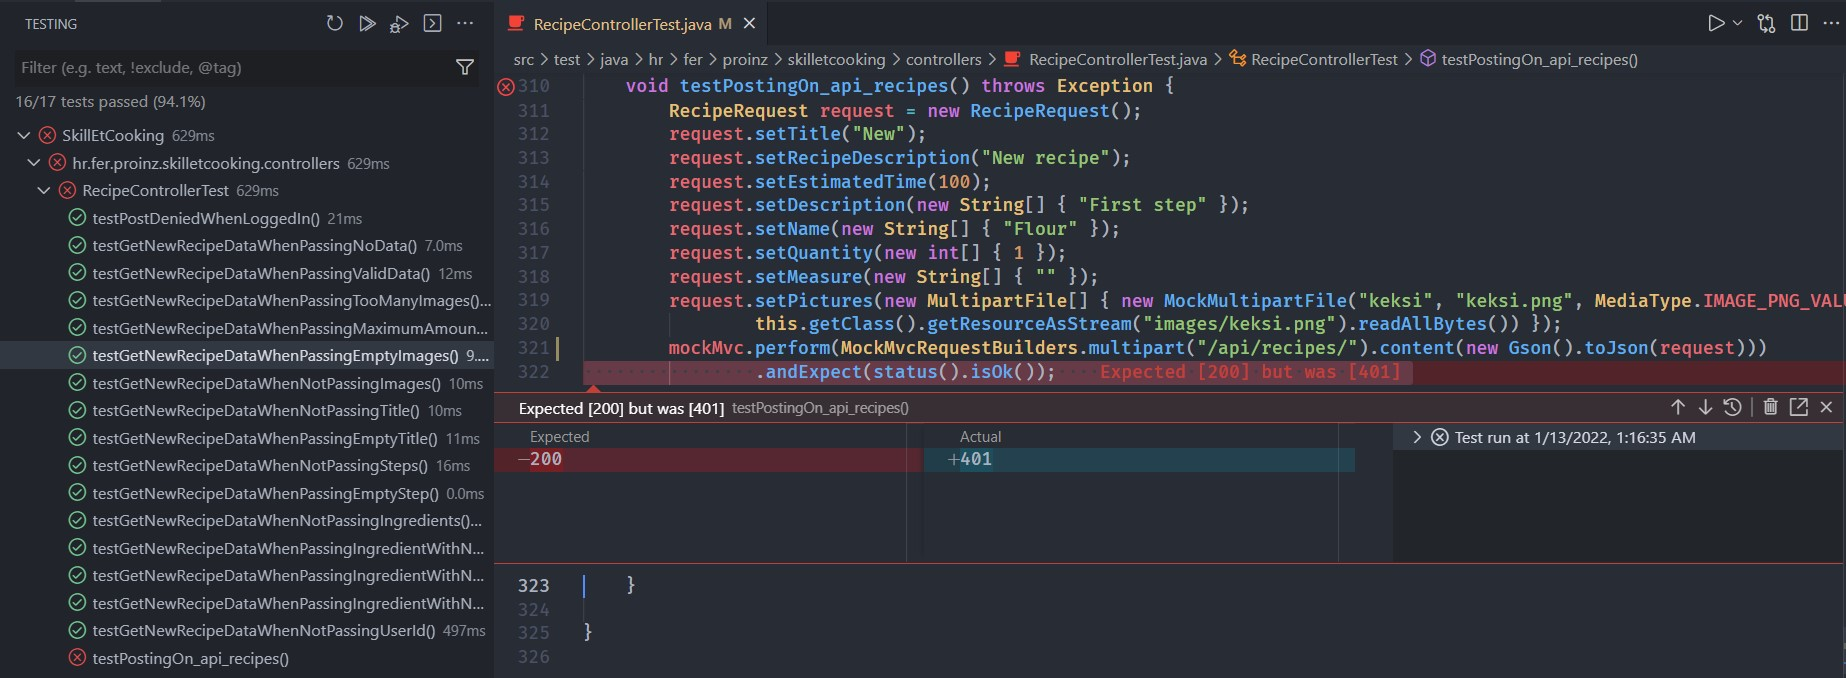
\includegraphics[scale=0.4]{slike/tests.jpg} %veličina slike u odnosu na originalnu datoteku i pozicija slike
	\centering
	\caption{Rezultati izvođenja testova u uređivaču VSCode.}
	\label{fig:promjene}
\end{figure}

\subsection{Ispitivanje sustava}
\noindent \underbar{\textbf{1. Ispitivanje prijave u sustav (UC-7)}}\break
U ovom ispitnom slučaju je provedena prijava. Scenarij započinje otvaranjem početne stranice i pod pretpostavkom da korisnik
nije prijavljen u sustav biti će vidljiva hiperveza koja vodi na stranicu za prijavu. Nakon toga unošenjem korisničkog imena
i lozinke te klikom na gumb za prijavu korisnik bi trebao biti preusmjeren na početnu stranicu ali ovaj put uz dodatne mogućnosti
što se provjerava postojanjem hiperveze koja vodi na vlastite recepte.
\begin{figure}[H]
	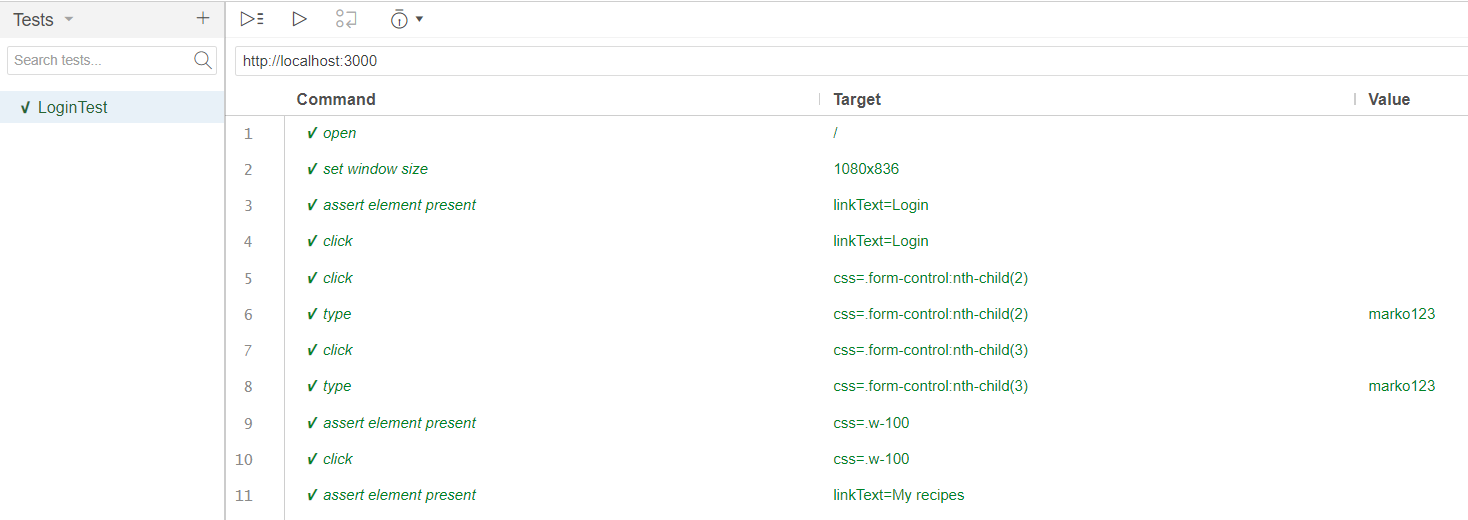
\includegraphics[scale=0.6]{slike/login.png} %veličina slike u odnosu na originalnu datoteku i pozicija slike
	\centering
	\caption{Ispitivanje prijave u sustav.}
	\label{fig:promjene}
\end{figure}

\noindent \underbar{\textbf{2. Ispitivanje pretraživanja recepta po sastojcima (UC-5)}}\break
U ovom ispitnom slučaju je provedeno pretraživanje recepata po sastojcima. Scenarij započinje
otvaranjem početne stranice na kojoj se nalazi HTML element za unos sastojaka. Pod pretpostavkom
da u bazi postoji recept sa sastojcima: peršin, češnjak, špageti i vrhnje (za-kuhanje),
nakon odabira upravo tih sastojaka na početnoj stranici bi trebao biti vidljiv taj recept što se
provjerava njegovom prisutnošću.
\begin{figure}[H]
	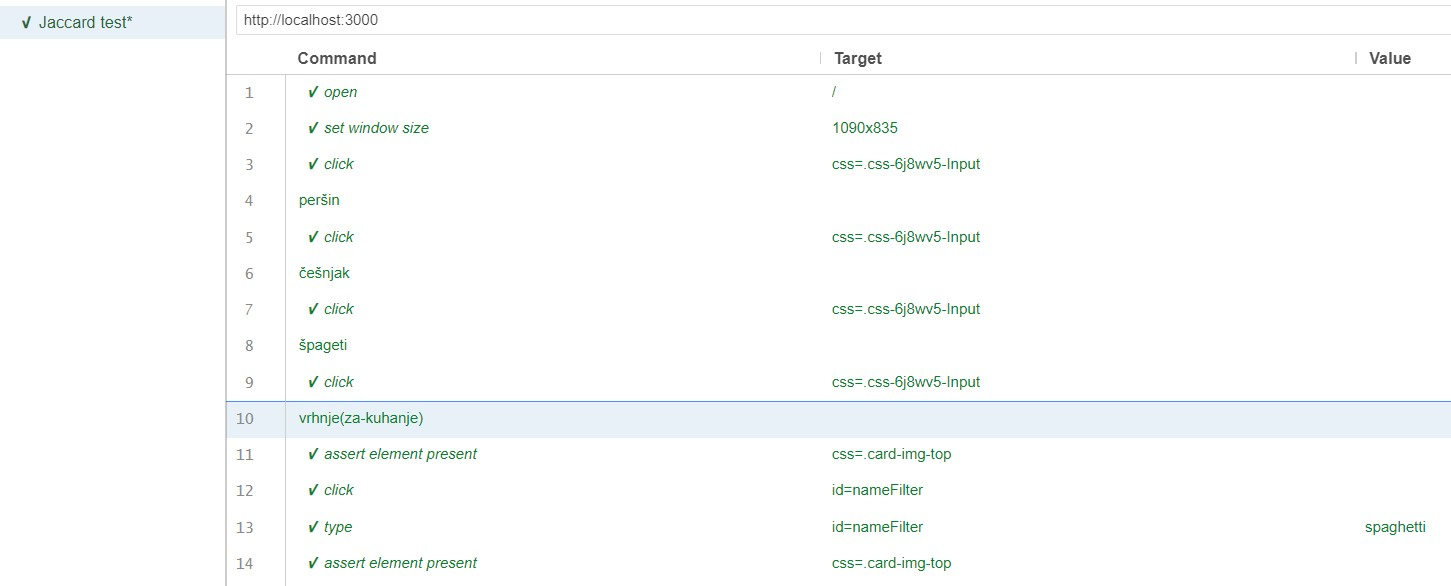
\includegraphics[scale=0.6]{slike/jaccard.jpg} %veličina slike u odnosu na originalnu datoteku i pozicija slike
	\centering
	\caption{Ispitivanje pretraživanja recepata po sastojcima.}
	\label{fig:promjene}
\end{figure}

\newpage

\noindent \underbar{\textbf{3. Ispitivanje registracije u sustav (UC-6)}}\break
U ovom ispitnom slučaju je provedena registracija korisnika u sustav. Scenarij započinje otvaranjem početne
stranice gdje su prikazani svi recepti. Nakon toga korisnik odabire hipervezu registracija koja
ga vodi na formu za registraciju. Korisnik popunjava podatke te ako su zadovoljeni svi uvjeti
korisnik će biti uspješno registriran te će ga se potom preusmjeriti na početnu stranicu,
ali će ovaj put biti prijavljen u sustav. Nakon toga će biti vidljiva hiperveza My recipes
koja se pojavljuje samo prijavljenim korisnicima.
\begin{figure}[H]
	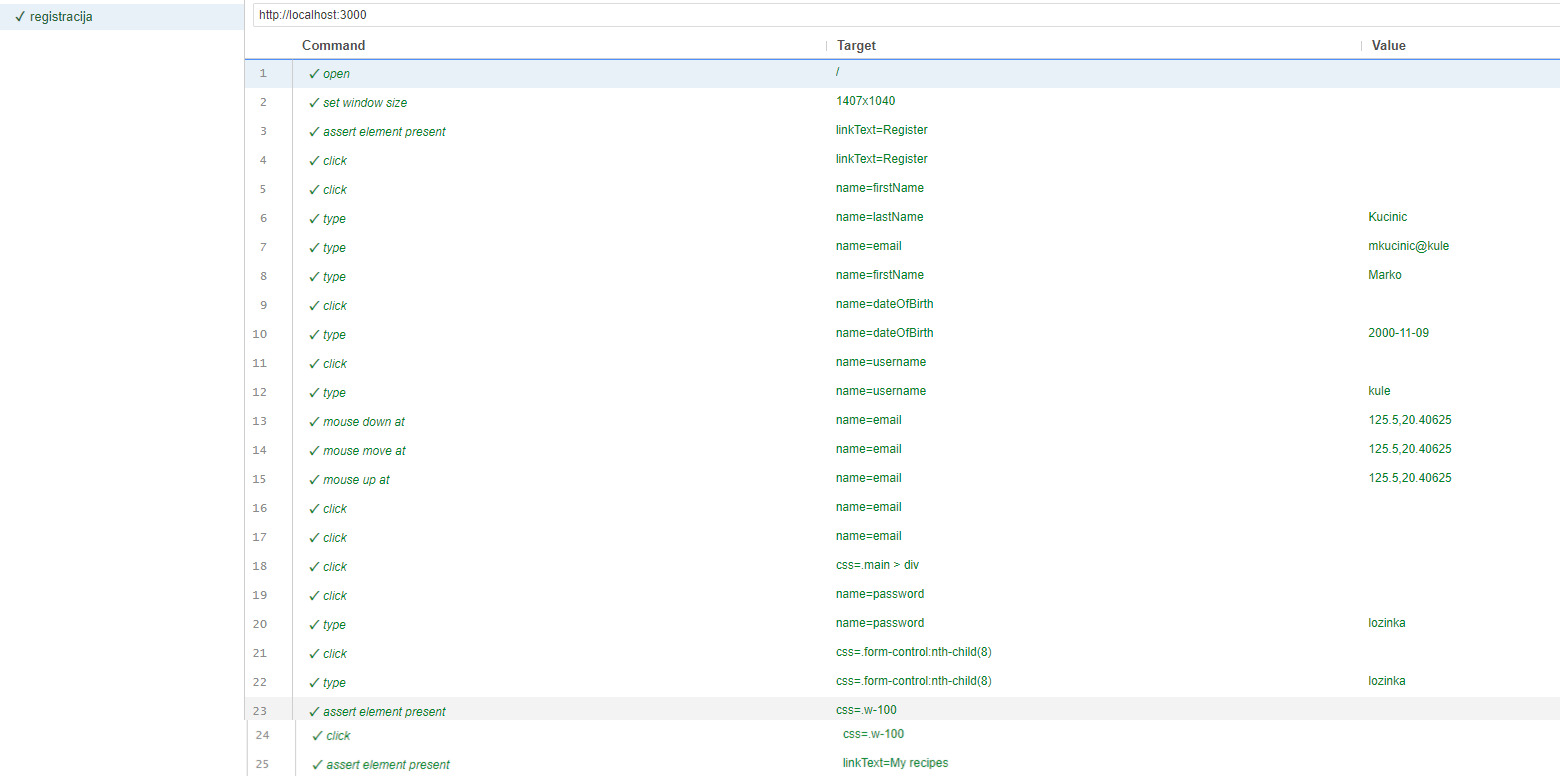
\includegraphics[scale=0.2]{slike/registracija1.png} %veličina slike u odnosu na originalnu datoteku i pozicija slike
	\centering
	\caption{Ispitivanje registracije u sustav.}
	\label{fig:promjene}
\end{figure}

\noindent \underbar{\textbf{4. Ispitivanje dodavanja komentara moderatora (UC-14)}}\break
U ovom ispitnom slučaju je provedeno dodavanje komentara moderatora. Moderator se poput ostalih
korisnika mora prijaviti u sustav. Nakon prijave moderator odabire opciju prikaza određenog
recepta. U polju za komentare upisuje komentar po želji i pritiskom na hipervezu objavi
komentar dodaje komentar u bazu. Pritiskom na tipku osvježi komentar će se prikazati uz
ostale komentare toga recepta. Također, komentar će biti dodatno naglašen oznakom za moderatore (kruna).
\begin{figure}[H]
	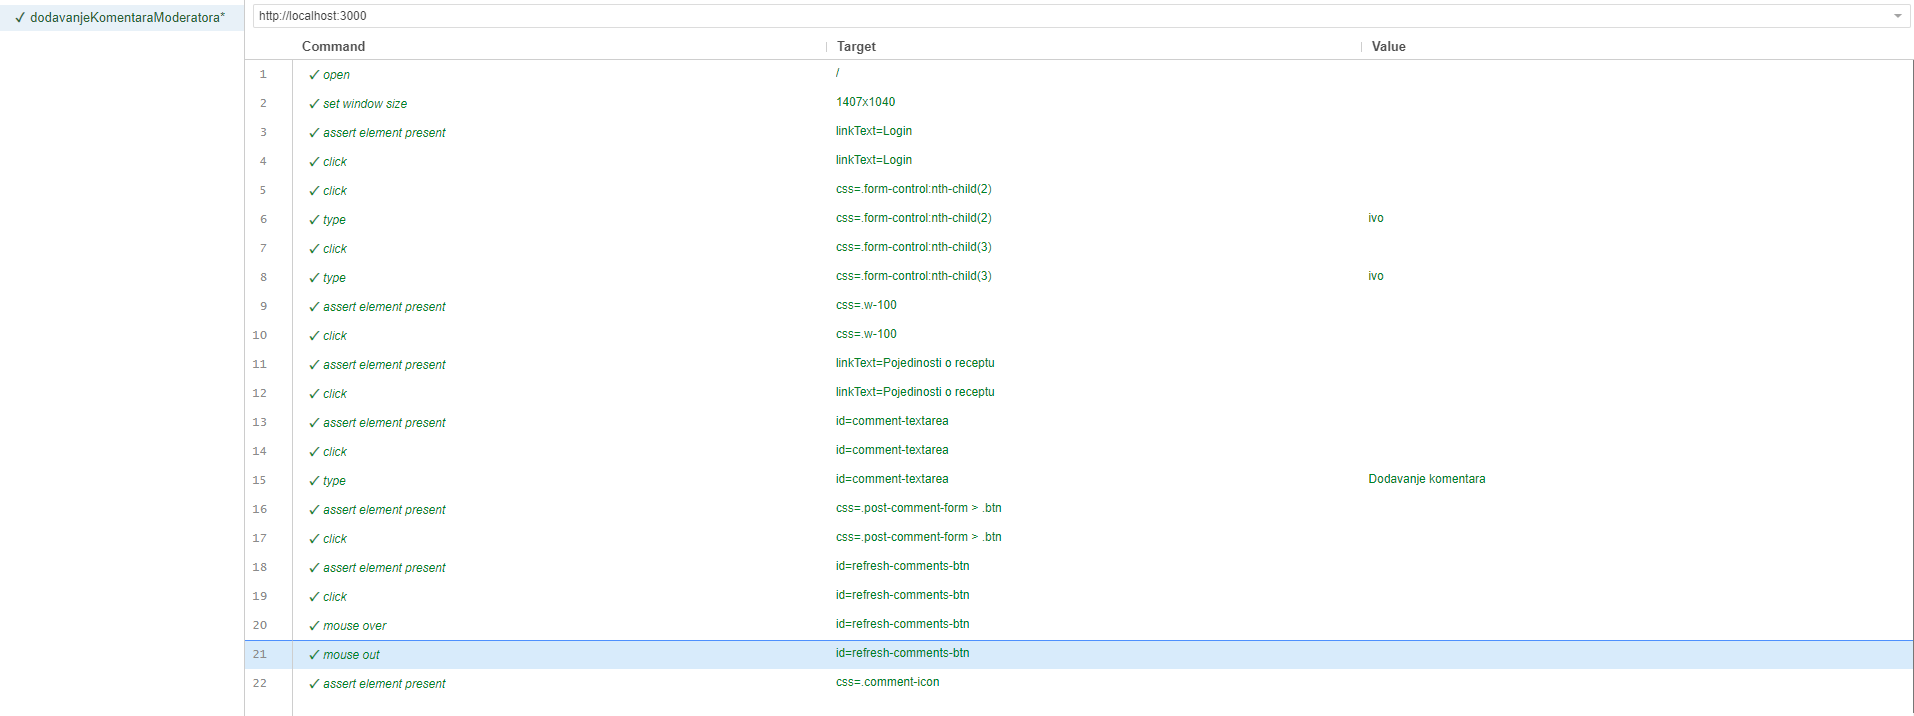
\includegraphics[scale=0.4]{slike/dodavanjeKomentaraModeratora.png.jpg} %veličina slike u odnosu na originalnu datoteku i pozicija slike
	\centering
	\caption{Ispitivanje dodavanja komentara moderatora.}
	\label{fig:promjene}
\end{figure}

\eject


\section{Dijagram razmještaja}

Dijagrami razmještaja opisuju topologiju sklopovlja i programsku potporu koja se koristi u implementaciji sustava u njegovom radnom okruženju. Upogonjenje smo izvršili na AWS-u pa imamo dijagram s 3 uređaja. Servis web poslužitelja pokrenut je na Amazon EC2 instanci koji s bazom pokrenutoj preko Amazon RDS-a komunicira preko TCP protokola na vratima 5432. Klijenti koriste web preglednik na vlastitim računalima kako pi pristupili web aplikaciji. Sustav je baziran na arhitekturi "klijent -poslužitelj", a komunikacija između računala korisnika i poslužitelja odvija se preko HTTP veze.
\begin{figure}[H]
	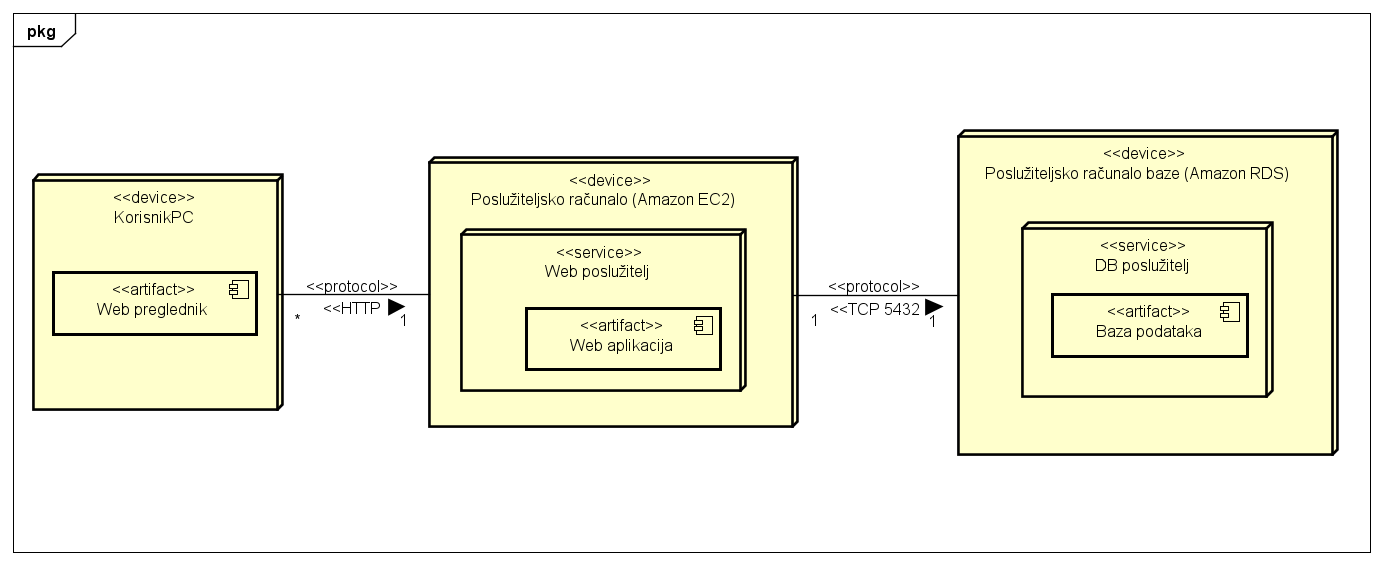
\includegraphics[scale=0.45]{slike/DijagramRazmjestaja.PNG} %veličina slike u odnosu na originalnu datoteku i pozicija slike
	\centering
	\caption{Dijagram razmještaja}
	\label{fig:promjene}
\end{figure}
\eject

\section{Upute za puštanje u pogon}

\lstset{
	backgroundcolor=\color{white},   % choose the background color; you must add     \usepackage{color} or \usepackage{xcolor}; should come as last argument
	basicstyle=\footnotesize,        % the size of the fonts that are used for the code
	breakatwhitespace=false,         % sets if automatic breaks should only happen at whitespace
	breaklines=true,                 % sets automatic line breaking
	captionpos=t,                    % sets the caption-position to top
	deletekeywords={...},            % if you want to delete keywords from the given language
	escapeinside={\%*}{*)},          % if you want to add LaTeX within your code
	extendedchars=true,              % lets you use non-ASCII characters; for 8-bits encodings only, does not work with UTF-8
	frame=single,                      % adds a frame around the code
	keepspaces=true,                 % keeps spaces in text, useful for keeping indentation of code (possibly needs columns=flexible)
	keywordstyle=\color{blue},       % keyword style
	morekeywords={*,...},            % if you want to add more keywords to the set
	rulecolor=\color{black},         % if not set, the frame-color may be changed on line-breaks within not-black text (e.g. comments (green here))
	showspaces=false,                % show spaces everywhere adding particular underscores; it overrides 'showstringspaces'
	showstringspaces=false,          % underline spaces within strings only
	showtabs=false,                  % show tabs within strings adding particular underscores
	tabsize=2,                     % sets default tabsize to 2 spaces
	title=\lstname                   % show the filename of files included with \lstinputlisting; also try caption instead of title
}
\hfill \break
\textbf{Instalacija potrebnih programa}\\
Prije lokalnog pokretanja potrebno je instalirati sljedeće programske alate:
\begin{itemize}
	\item Node + NPM
	\item Java 11
	\item Maven
	\item PostgreSQL 12 + PgAdmin
	\item git
\end{itemize}

Za kloniranje repozitorija i koda koristimo sljedeću naredbu te se autenticiramo našim GitLab podacima:
\begin{lstlisting}[]
git clone https://gitlab.com/progimeri/proinz-projekt.git
\end{lstlisting}
\hfill \break
\hfill \break
\textbf{Konfiguracija baze podataka}\\

Prije pokretanja same web aplikacije moramo konfigurirati lokalnu bazu podataka. Konfiguraciju poslužitelja baze možemo napraviti proizvoljno te poslije specificirati u kodu, ali preporuča se korištenje zadanih podataka:
\begin{figure}[H]
	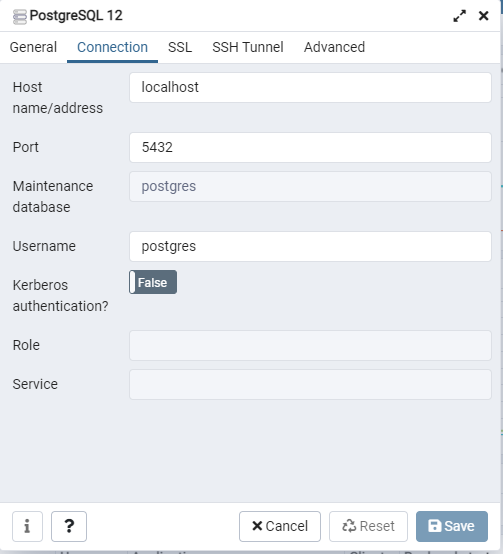
\includegraphics[scale=1]{slike/server_properties.PNG} %veličina slike u odnosu na originalnu datoteku i pozicija slike
	\centering
	\caption{Postavke poslužitelja baze}
	\label{fig:promjene}
\end{figure}
Nakon stvaranja poslužitelja baze možemo stvoriti bazu bilo kojeg imena, ali preporuka je koristiti ime 'skilletcooking' s vlasnikom 'postgres':
\begin{figure}[H]
	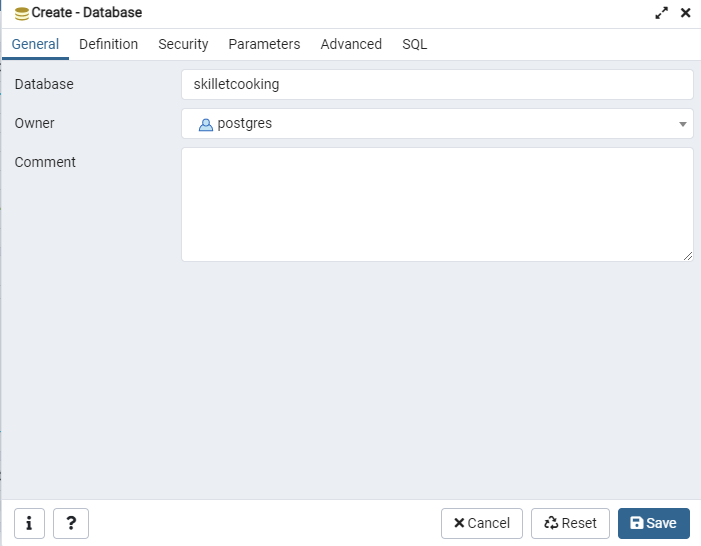
\includegraphics[scale=0.8]{slike/database_properties.PNG} %veličina slike u odnosu na originalnu datoteku i pozicija slike
	\centering
	\caption{Postavke baze podataka}
	\label{fig:promjene}
\end{figure}
\hfill \break
\textbf{Konfiguracija stražnjeg dijela}\\
Samu shemu baze popuniti će Flyway migracija prilikom prvog pokretanja back-end poslužitelja. Kako bi poslužitelj spojili na lokalnu bazu podataka trebamo definirati da je aktivni profil dev u application.properties datoteci:
\begin{lstlisting}
spring.profiles.active=dev
\end{lstlisting}

Samim time ako se zbog nekog razloga želimo spojiti na bazu podataka koja je pokrenuta na AWS-u to možemo jednostavno tako da zamijenimo aktivni profil sa prod:
\begin{lstlisting}
spring.profiles.active=prod
\end{lstlisting}

Prijašnje postavke koje smo definirali pri izradi baze podataka sada moramo specificirati u application-dev.properties datoteci u izvornom kodu back-enda i izmijeniti sljedeće linije.
\lstset{}
\begin{lstlisting}[]
spring.datasource.url=jdbc:postgresql://{host_name}/{database_name}
spring.datasource.username={database_user_name}
spring.datasource.password={lozinka}

spring.flyway.url=jdbc:postgresql://{host_name}/{database_name}
spring.flyway.user={database_user_name}
spring.flyway.password={lozinka}
\end{lstlisting}

Za predložene podatke i korisnika postgres kojemu je lozinka 'bazepodataka' to bi izgledalo ovako:
\begin{lstlisting}[]
spring.datasource.url=jdbc:postgresql://localhost:5432/skilletcooking
spring.datasource.username=postgres
spring.datasource.password=bazepodataka

spring.flyway.url=jdbc:postgresql://localhost:5432/skilletcooking
spring.flyway.user=postgres
spring.flyway.password=bazepodataka
\end{lstlisting}
Kada je cijela konfiguracija namještena napokon možemo pokrenuti back-end koji će pokrenuti generiranje sheme u bazi. To možemo tako da se u konzoli pozicioniramo u mapu izvorniKod/back-end i pokrenemo naredbu \lstinline|mvn spring-boot:run| koja će pokrenuti Java Spring poslužitelj na vratima 8080. Back-end se također može pokrenuti korištenjem modernih naprednih IDE-jeva poput IntelliJ-a.\\
Kada je servis uspješno pokrenut i nakon popunjenja sheme još jedan preduvjet prije pokretanja cjelokupne aplikacije je definicija "uloga" koje korisnici mogu imati, a to su \textbf{USER} i \textbf{MODERATOR}. Te uloge možemo jednostavno dodati korištenjem alata za upite u PgAdminu i pokretanju sljedećih upita:
\begin{lstlisting}[language=sql]
INSERT INTO roles(role_name) VALUES ('USER');
INSERT INTO roles(role_name) VALUES ('MODERATOR');
\end{lstlisting}
\textbf{Pokretanje prednjeg dijela}\\
Sada je cijeli back-end spreman i možemo pokrenuti front-end. Pokrenimo novu konzolu i pozicioniramo se u mapu izvorniKod/front-end. Pokrećemo naredbu \lstinline|npm install| koja će instalirati sve potrebne pakete s npm-a te nakon toga možemo izvršiti naredbu \lstinline|npm start| koja će pokrenuti poslužitelj za prednju stranu na vratima 3000 i njemu možemo pristupiti na adresi localhost:3000.

\hfill \break
\textbf{Javni poslužitelj}\\
Aplikacija je pokrenuta na javnom poslužitelju preko AWS-a i dostupna je na stranici: http://34.244.45.75/ .
\eject